\chapter{绪论}\thispagestyle{main}
\section{课题背景}
\par 我们正处在海量数据和大数据的时代,数字电视、摄像机以及其他通讯技术的出现正快速的加剧着数据的增长。据 IDC(国际数据中心International Data Center)统计,2007年数字内容总量第一次超过了全球存储总容量,并且每年数据总量以指数的速度不断增长[1]。数据的爆炸性的增长给大型企业的数据中心带来了较大的压力,以不断扩大甚至扩建数据中心的方式并不能有效的缓解需要存储的数据的增长速度。同时,随着科技的快速发展和信息化的全面普及,数据对于企业甚至国家越来越重要,对于银行和互联网等公司,数据是它们赖以生存的根本,决定着未来的命运。
\par 但是,由于种种未知的原因,人们无法预知或者避免数据的丢失和损坏。例如恐怖事件、系统故障、人为操作、自然灾害、黑客攻击、计算机病毒等各种因素,时刻威胁着大量对企业和国家至关重要的数据。在1993 年,美国世贸中心由于恐怖袭击发生爆炸。在爆炸前,大约有 350 家企业在该大楼中办公,然而一年后,世贸大楼的公司只剩下了150 家,其余的 200 家公司由于无法获取原有的重要数据而被迫倒闭。 根据Gartner Group 的数据表明,企业数据灾难导致很多公司停止运营,其中2/5的公司无法再重新恢复,剩下的也有1/3在两年内相继宣告破产。
\par 重复数据删除技术是一种新型的高级的数据压缩方式,它通过识别出重复的数据部分,删除冗余的部分,是一种更有效的节省磁盘空间的方法。研究发现,在数据备份系统中所存储的数据中有高达60\%的数据是冗余的,而且这一比例会逐渐增加。
\par 因此,基于重复数据删除技术的备份系统,对于节省磁盘空间、减少网络带宽、缩短恢复窗口期等有很重要的理论意义和实际意义。
\section{国内外研究现状}
\par 重复数据删除技术作为一种有效的数据压缩方法被存储界列为十大存储热门技术之一,最早是由美国的\ \ Data Domain\ \ 公司提出来的。在数据备份和归档领域得到了广泛的运用,由于基于重复数据删除技术的备份系统能够取得较好的压缩率以及性能,以及相应的带来的节省带宽、降低成本等效益,重复数据删除技术越来越受到学术界和工业界的关注,成为存储界的一大新兴技术热点,并在高校和企业广泛研究和应用,并且取得了一系列的成果。
\par 以上排版与《重复数据删除技术的实现与优化》一致
\section{简单的数学公式和定理}
\begin{sthm}[定理~\thethm~(存在性定理)]
$\Gamma\Theta\Lambda\Xi\Pi\alpha\beta\gamma\delta$
\end{sthm}

\begin{thm}\label{thm:alpha}
xxxxx
\end{thm}
\begin{equation}\label{equ:alpha}
\alpha=\sqrt[n]{\Re}.
\end{equation}
\par 定理\ref{thm:alpha},公式\ref{equ:alpha}

\section{参考文献}
参考文献\cite{broder1997resemblance}\cite{broder1997syntactic}

\section{图片}
\begin{figure}
  \centering
  % Requires \usepackage{graphicx}
  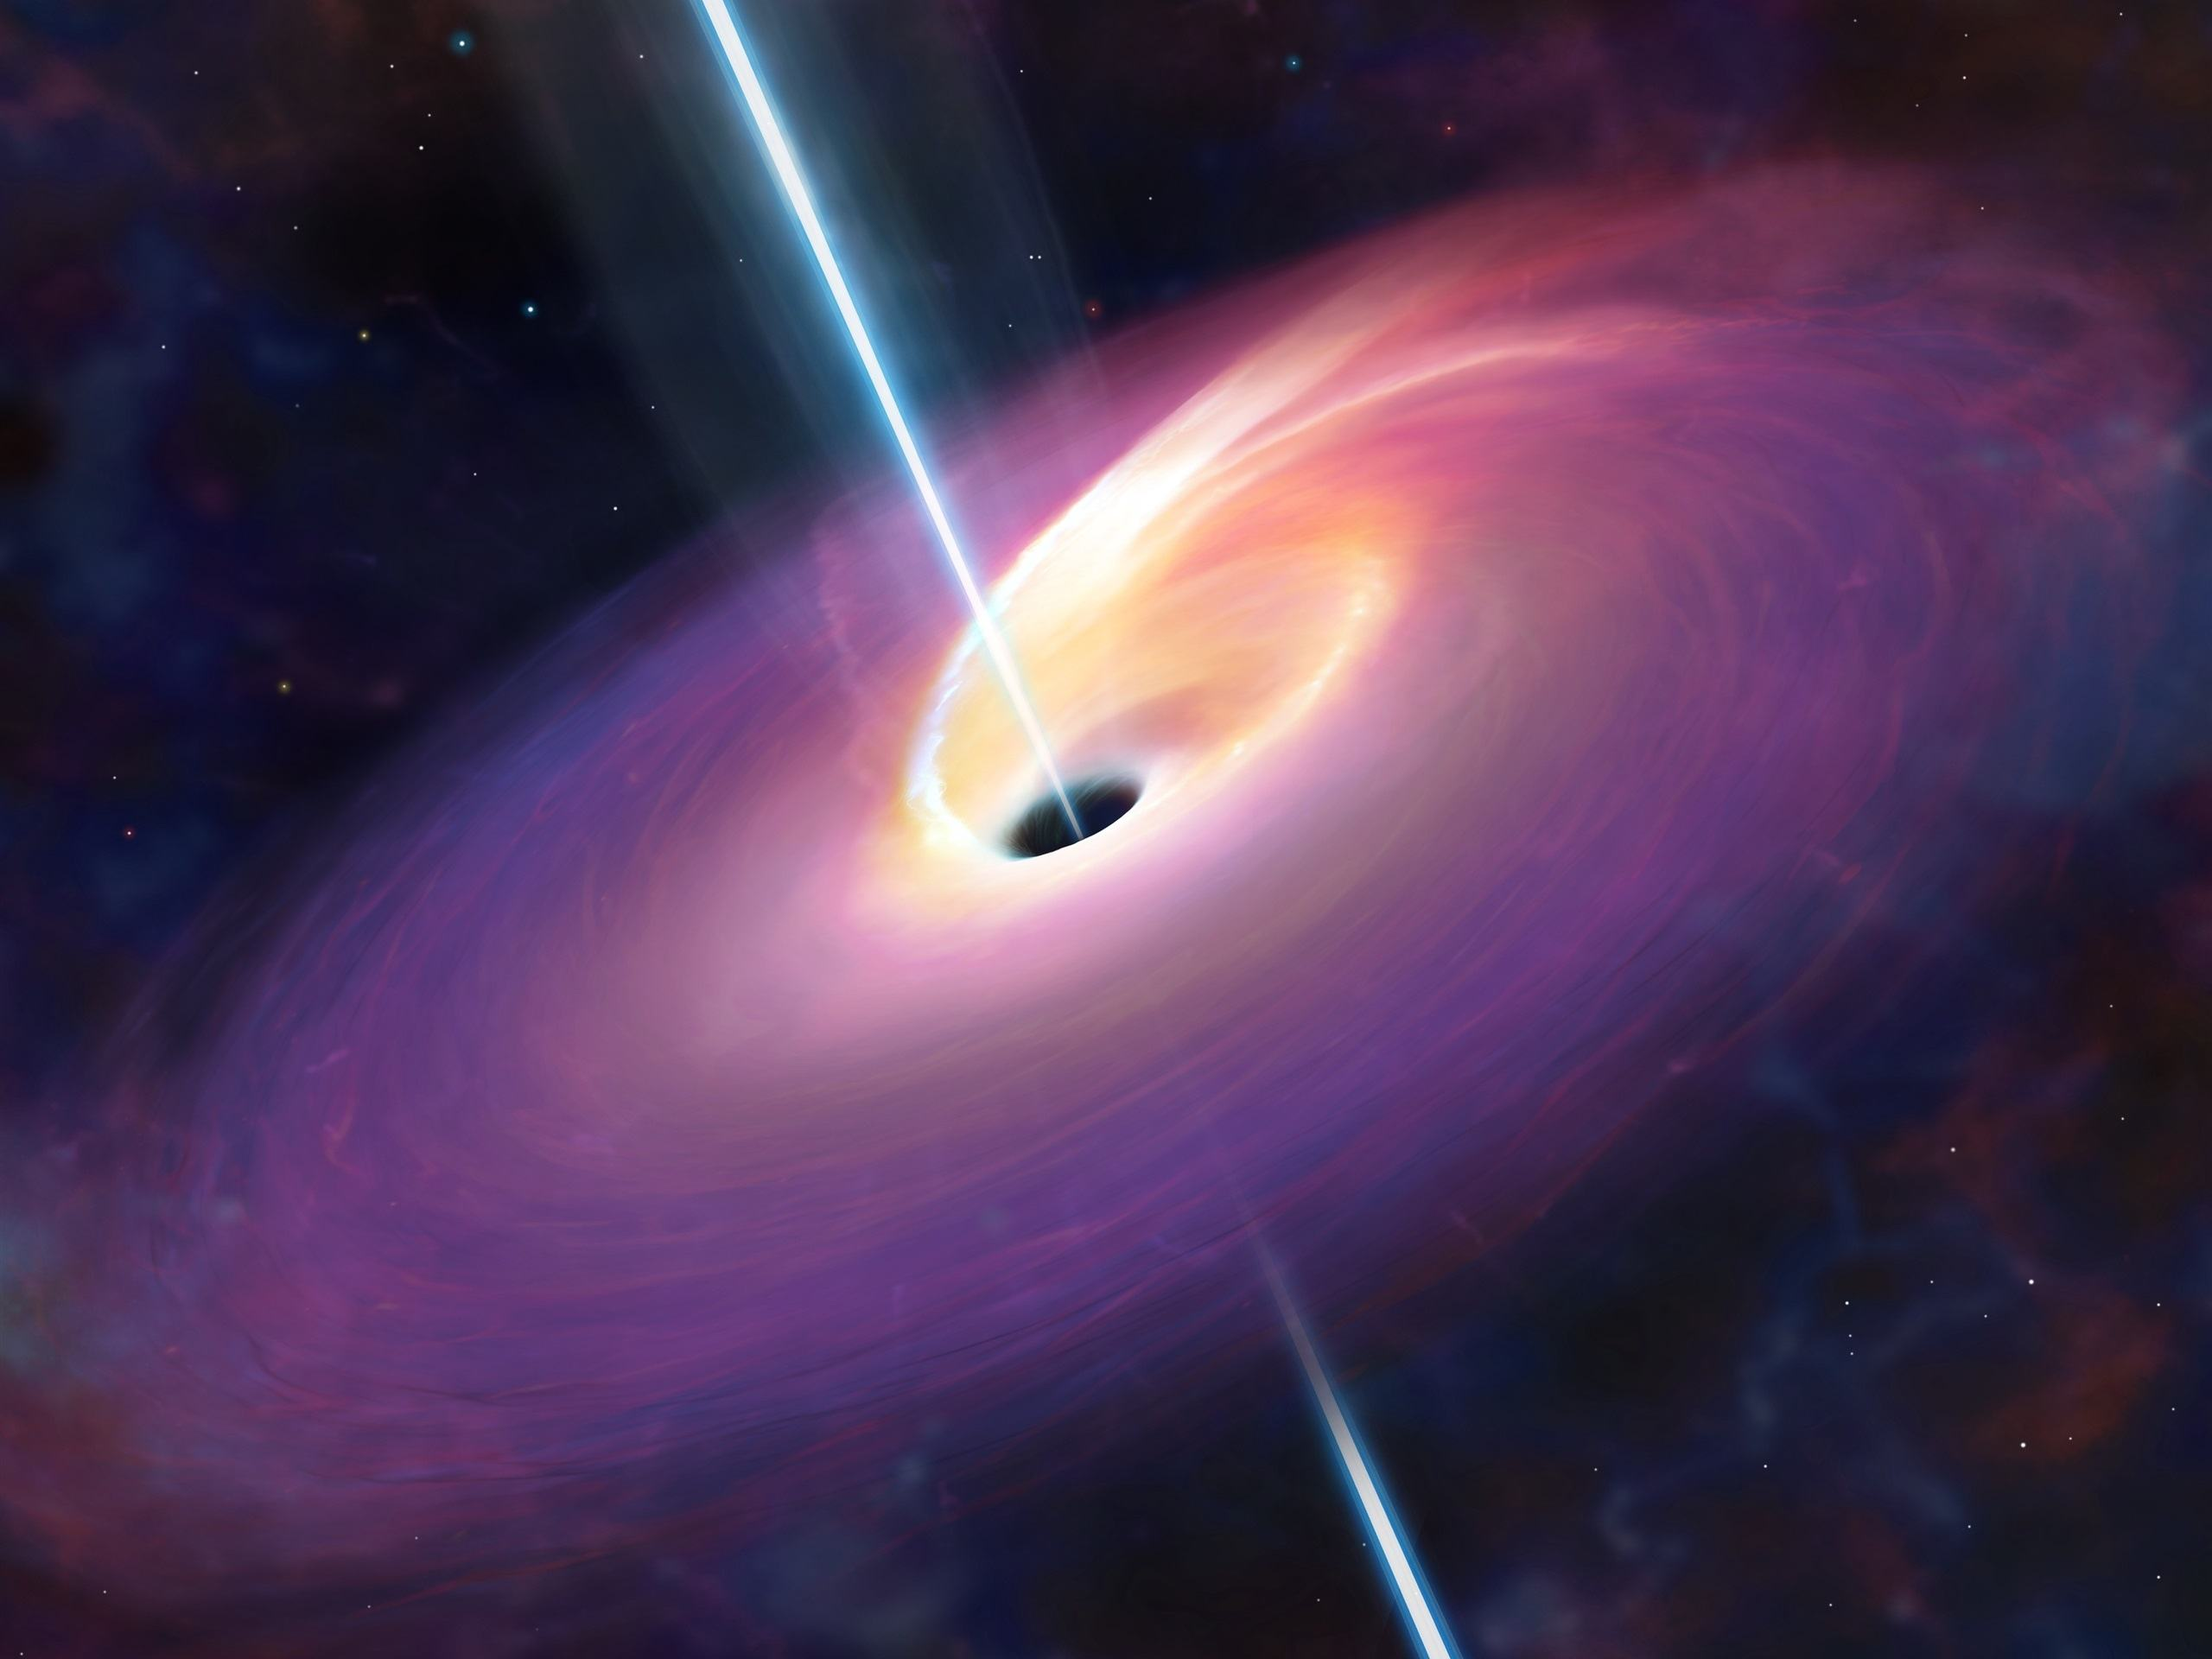
\includegraphics[width=2.5in]{images/blackhole.jpeg}\\
  \caption{黑洞}\label{img:logo}
\end{figure}
图\ref{img:logo}是黑洞。
\section{表格}
\begin{table}[!t]
    \centering
    \caption{一个表的实例}\label{table:tabobj}
    \renewcommand{\arraystretch}{1.5}
    \begin{tabular}{
    p{0.1\textwidth}<{\centering}p{0.1\textwidth}<{\centering}
    p{0.1\textwidth}<{\centering}p{0.1\textwidth}<{\centering}
    p{0.1\textwidth}<{\centering}}
        \Xhline{1.2pt}
         r1   &r2         &r3       &r4   &r5\\
        \Xhline{1.2pt}
        $4KB$                   &128929s   &106511s &128201s    &128201s\\
        \Xhline{1.2pt}
    \end{tabular}
\end{table}
表\ref{table:tabobj}是一个实例。
